\section{pSAIS}
\label{section:psais}

\currentauthor{Jonas Bode} 

Der pSAIS -- kurz für \textbf{parallel SAIS} -- ist ein SACA, der sich aus dem SAIS entwickelt hat und mithilfe von parallel laufenden Threads ein Suffixarray berechnet \cite{psais}. Die grundlegende Idee des pSAIS ist es, das SA für das Induced Sorting zuerst in mehrere Blöcke aufzuteilen mit Blockgröße $\beta$ (diese wurde in unserer Implementierung fest auf 10 MiB gesetzt). Für diese Blöcke kann die Methode des Induced Sortings dann teilweise parallelisiert werden. Das Framework des pSAIS entspricht dabei dem des SAIS bis auf die hier aufgeführten Veränderungen und Neuerungen. \\
Es werden Buffer-Listen $r$ und $w$ für das Lesen aus dem Text und das Schreiben in das \textit{SA}  eingeführt, welche die selbe Länge $\beta$ haben und Tupel der Art $\langle chr, pos \rangle$ bzw. $\langle idx, pos \rangle$ enthalten. In dem Lese-Buffer $r$ gibt $chr$ ein Zeichen des Textes und $pos$ seine Position im Text an. In dem Schreib-Buffer $w$ ist $pos$ eine Position im Text und $idx$ ist die Position des SAs, an welcher $pos$ eingeordnet werden soll. Für jeden Block $B$ werden dann die folgenden drei Phasen nacheinander durchgeführt:

\begin{itemize}
\item \textbf{Preparing:} Hier werden alle Paare $\langle chr, pos \rangle$ in einen Lese-Buffer $r$ hineingeschrieben, welche die Bedingung erfüllen, dass $pos = B[j]-1$ ist, für eine Position $j$ von Block $B$. Je nachdem um welches Induce Sorting es sich handelt muss $\inputtext[pos]$ außerdem ein L- bzw. S-Typ sein. Das gesamte Preparing wird hierbei \textbf{parallel} für jede Stelle $j$ des Blocks $B$ aufgerufen. Das Preparing lädt also bestimmte Zeichen in den Lese-Buffer, welche dann in dem folgenden Schritt effizient und ohne direkt auf den Text zugreifen zu müssen herausgelesen werden können.

\item \textbf{Inducing:} Das Induzieren folgt auf das Preparing des Blockes $B$. Es erfolgt \textbf{nicht parallel} und benutzt den vorher beschriebenen Read-Buffer $r$. Block $B$ wird durchlaufen und für jede Position $i$ in $B$ wird wie beim Induced Sorting überprüft, ob $chr = B[i]-1$ ein L- bzw. ein S-Typ ist. Falls dem so ist, wird die in $r[i].chr$ gespeicherte Information benutzt um direkt das passende Zeichen zu dieser Position zu erhalten. Ist $r[i]$ leer -- dies kann z.B. passieren wenn $B[i]-1$ gar nicht mehr in Block $B$ hineingehört -- wird stattdessen das Zeichen aus dem Text gelesen, also $\inputtext[B[i]-1]$. Danach wird zu dem gelesenen Zeichen die passende Position $pos$ für $chr$ im SA gesucht und das Tupel $\langle chr, pos \rangle$ wird in einen Schreib-Buffer $w$ eingefügt, falls $pos$ in den Bereich des momentanen Blocks $B$ oder den des darauffolgenden Blocks $B^\prime$ fällt. Fällt $pos$ nicht in den Bereich einer der beiden Blöcke, wird direkt in das SA geschrieben: $SA[pos] = chr$.

\item \textbf{Updating:} Im Updating wird \textbf{parallel} der Schreib-Buffer $w$ durchlaufen und für jedes Paar $\langle chr, pos \rangle$ in $w$ wird $SA[pos] = chr$ gesetzt. Das Updating hilft, genau wie das Preparing, die Zugriffe auf das SA bzw. den Eingabetext effizienter zu machen, da andernfalls bei direkten Zugriffen viele Cache Misses entstehen können.
\end{itemize}

Diese drei Stufen, welche wir das \textbf{Pipelined Inducing} nennen, ersetzen vollständig das Induzieren im pSAIS. Wird SA in die Blöcke $B_0, \ldots, B_m-1$ eingeteilt, so müssen für das Induzieren der L-Typen die Blöcke in der angegebenen Reihenfolge durchlaufen werden, für das Induzieren der S-Typen müssen sie jedoch in umgekehrter Reihenfolge durchlaufen werden. Wir stellen dafür im Folgenden in \ref{pipL} nur das Pipelined Inducing der L-Typen dar, da sich das Pipelined Inducing der S-Typen daraus herleiten lässt.

\begin{figure}
\begin{minted}[escapeinside=@@,numbers=left]{python}
def pipelined_l_inducing(T, k, t, BA, SA):
# Input text T
# Blocknumber k
# Type Array t
# Bucket Counter Array BA
# Suffixarray SA with LMS suffixes already sorted in

# Parallel: Preparing
parallel for @$i = 0$@ to @$\beta-1$@ do 
   Initialize r and w as empty
   j = k * @$\beta$@ + i 	       # Global current Position in T
   if (SA[j] is non-empty and (pos = SA[j]-1) @$\leq$@ 0 and t[pos] is L-Type)
    @$chr$@ = T[pos]
    Insert @$\langle chr, pos \rangle$@ into r[i]
		
# Sequential: Inducing
for @$i = 0$@ to @$\beta-1$@ do 
 if (B@$_k$@[i] is non-empty and (pos = B@$_k$@[i] -1)  @$\leq$@ 0 and t[pos] is L-Type)
  if (r[i].chr is empty)
   @$chr$@ = T[pos]
  else
   @$chr$@ = r[i].@$chr$@ # preceding character was already stored in read buffer
idx = BA[@$chr$@]++
if(idx is in Block B@$_k$@ or B@$_{k+1}$@)
 Write SA[idx] = pos
else
 Insert @$\langle idx, pos \rangle$@ into w[i]
 
# Parallel: Updating
parallel for @$i = 0$@ to @$\beta-1$@ do
 if w[i] is non-empty then
  SA[w[i].idx] = w[i].pos


\end{minted}
\caption{Pipelined L-Inducing nach \cite{psais}}
\label{pipL}
\end{figure}

\subsection{Verschränktes Induzieren}

Eine weitere Technik des pSAIS, um viele Berechnungsschritte parallel machen zu können, ist das gleichzeitige Ausführen einiger Schritte des Pipelined Inducings für aufeinander folgende Blöcke. Um dies möglich zu machen, werden je zwei anstatt nur je ein Lese- und Schreibbuffer benutzt. Diese Buffer nennen wir $r_1, r_2$ bzw. $w_1, w_2$. Ein Pipelined-Inducing Vorgang für einen festen Block $B_i$ verwendet dabei immer die selben Lese- und Schreibbuffer $w_j, r_j$. Der darauffolgende Block $B_{i+1}$ verwendet jedoch die Buffer $w_{\bar j}, r_{\bar j}$, mit $\bar j = 3 - j$, also genau die vom Block $B_i$ nicht benutzten Buffer. So können die folgenden Teile des Pipelined Inducings parallel berechnet werden:

\begin{itemize}
\item Während das Inducing des Blockes $B_i$ mit den Buffern $r_j, w_j$ ausgeführt wird, kann das Preparing des Blockes $B_{i+1}$ mit dem Buffer $r_{\bar{j}}$ ausgeführt werden.
\item Während das Updating des Blockes $B_i$ mit dem Buffer $w_j$ ausgeführt wird, kann das Inducing des Blockes $B_{i+1}$ mit den Buffern $r_{\bar{j}}, w_{\bar{j}}$ ausgeführt werden.
\end{itemize}

Eine graphische Darstellung dieses Prozesses findet sich unter Abbildung \ref{psaisArch}.

\begin{figure}
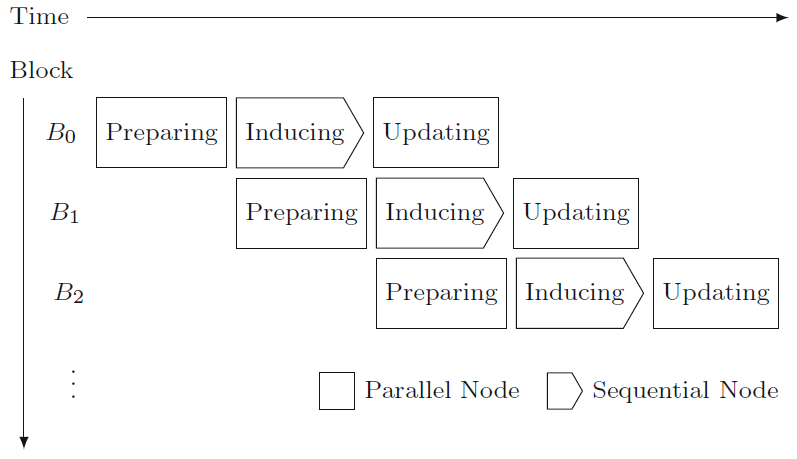
\includegraphics[width=\textwidth]{kapitel/saca_algorithmen/psais/psais_architecture.png}
\caption{Graphische Darstellung des verschränkten Induzierens in \cite{psais}}
\label{psaisArch}
\end{figure}


\subsection{Parallele Substring-Benennung}

In \cite{psais} wird eine Methode gezeigt um das Benennen der LMS-Substrings vor dem Rekursionsaufruf zu parallelisieren. Dafür werden die geordneten Substrings in gleiche Blöcke zerteilt und für jeden Block wird ein Differenzen-Bitvektor berechnet. Für jeden Substring in dem Block, der verschieden von seinem nachfolgenden Substring ist, ist das zugeordnete Bit 1 in dem Vektor, andernfalls ist es 0. Aus den entstehenden Vektoren kann die Anzahl verschiedener Namen in diesem Block berechnet werden. Damit können die neuen Namen der jeweils ersten Substrings aller Blöcke sequentiell berechnet werden. Danach können parallel für jeden Block, ausgehend von dem bereits umbenannten ersten Substring des Blocks, die Namen der anderen Substrings des Blocks berechnet werden. \\

Diese Methode wurde in unserer Version des pSAIS aus Zeitmangel nicht implementiert. Die dort vorzufindende Art der Umbenennung erfolgt wie beim SAIS sequentiell.

\subsection{Paralleles Klassifizieren}\currentauthor{Christopher Poeplau}
\label{subsection:psais_classifying}

Um den SAIS auch beim initialen Klassifizieren zu beschleunigen, wird das Zuordnen von L- und S-Typen parallelisiert. Dabei wird der Text in Blöcke aufgeteilt, die selbständig von ihren Threads abgearbeitet werden. Um speichereffizient arbeiten zu können, werden die Typen in einen Bitvektor gespeichert. Das bedeutet die Threadgrenzen der Blöcke müssen immer einer Zweierpotenz entsprechen. Dies ist nötig, da die Datenstrukturen intern immer auf Bytes arbeiten und es beim Manipulieren der Bytes über Threadgrenzen hinweg zu \textit{Race-Conditions} kommen kann, das Ergebnis der Berechnung also davon abhängt, welcher Thread zuerst das jeweilige Byte bearbeitet.
Das parallele Klassifizieren funktioniert in zwei Durchgängen. 

Im ersten Durchgang klassifiziert jeder Thread seinen Block soweit es geht. Dabei ist es jedem Thread erlaubt, ein Zeichen über seinen eigenen Block zu schauen. Es ist ersichtlich, dass der letzte Thread, der den Block mit dem Sentinel bearbeitet, immer dazu in der Lage ist, seinen gesamten Block zu klassifizieren. Bei allen anderen Blöcken ist es möglich, dass sie kein oder nur einen Teil der Zeichen klassifizeren können. Jeder Thread speichert also zusätzlich bis zu welchem Zeichen er klassifizieren konnte. Falls er klassifizieren konnte, speichert er sich zusätzlich noch den klassifizierten Typ an der Threadgrenze, der für den zweiten Durchgang benötigt wird.
Exemplarisch für den ersten Durchgang folgt ein Beispiel. Der Einfachheit halber wurden die Threadgrenzen nach jeweils 4 Zeichen gesetzt und nicht byteweise:

\begin{center}
	\begin{tabular}{c|c|c|c}     
	           0     &             1         &           2          			&             3    \\   
          	aaaa     &          aaaa         &        aaba           			&          acc\$    \\            
         	xxxx     &          xxxx         &        SSLx           			&          SLLS     \\     
         	  x      &            x          &   \textbf{\textcolor{blue}{S}}            &          \textbf{\textcolor{red}{S}}      \\            	       
	\end{tabular}
\end{center}

Dadurch, dass das Sentinel das lexikographisch kleinstmögliche Zeichen ist und im pSAIS nur einmalig vorkommt, kann der 3. Block in seiner Gesamtheit klassifiziert werden. Der zweite Block versucht das letzte \textit{a} zu klassifizieren. Dies ist jedoch nicht möglich, da das nächste Zeichen auch ein \textit{a} ist. An dieser Stelle ist es noch nicht möglich, auf dessen Typ zuzugreifen und diesen zu übernehmen, da alle Threads gleichzeitig arbeiten und zu diesem Zeitpunkt nicht gewährleistet ist, dass der Typ schon geschrieben wurde. An den jeweiligen Stellen, die nicht klassifizert werden konnten steht ein x. Die Blöcke 0 und 1 konnten nichts klassifizieren, da auch mit dem nächsten Zeichen ihres Blocks keine Informationen über den Vorgängertypen ermitteln konnten. Alle Threads speichern zudem den ermittelten Typ an ihren Threadgrenzen. Da nur Block 2 und 3 klassifizieren konnten, steht nur bei ihnen kein x.

Im zweiten und finalen Durchgang des Klassifizierens werden die Informationen der benachbarten Blöcke genutzt, um den gesamten Text zu klassifizieren, der noch nicht klassifiziert werden konnte:

\begin{center}
	\begin{tabular}{c|c|c|c}      
		           0     	&             1         &           2           &             3    \\ 
          	aaaa     		&          aaaa         &        aaba           &          acc\$    \\            
\textbf{\textcolor{blue}{S}}\textbf{\textcolor{blue}{S}}\textbf{\textcolor{blue}{S}}\textbf{\textcolor{blue}{S}} &  \textbf{\textcolor{blue}{S}}\textbf{\textcolor{blue}{S}}\textbf{\textcolor{blue}{S}}\textbf{\textcolor{blue}{S}} & SSL\textbf{\textcolor{red}{S}}  & SLLS     \\             	       
	\end{tabular}
\end{center}

Im ersten Durchgang fehlte im Block 2 noch die Information, welchem Typ das \textit{a} entsprach. Diese Information ist nun vorhanden und das letzte Zeichen des Blocks kann klassifiziert werden. Das fettgedruckte rote \textit{S} konnte also durch die Information aus dem dritten Block klassifiziert werden. Analog verhält es sich mit den ersten beiden Blöcken, deren Zeichen alle S-Typen sind. Hier wird die Information aus dem zweiten Block auf die vorherigen beiden Blöcke übertragen.


